\begin{center}

\includegraphics[width=0.6\textwidth]{content/3/chapter5/images/29.png}\\
Cippi在做杯子
\end{center}

\begin{tcolorbox}[breakable,enhanced jigsaw,colback=blue!5!white,colframe=blue!75!black,title={缺少编译器支持}]
	
截止到2020年底,没有C++编译器支持格式化库。感谢Victor Zverovich的原型库\href{https://github.com/fmtlib/fmt}{fmt},我可以用它进行实验。该库托管在\href{https://godbolt.org/z/Eq5763}{Compiler Explorer}上。当三大编译器GCC、Clang或MSVC中的一个支持C++20格式库,我将修改本章中的示例,使其使用标准库。
	
\end{tcolorbox}

格式化库为替代\href{https://en.cppreference.com/w/cpp/io/c/fprintf}{printf}系列函数提供了一种安全且可扩展的方案,并扩展了I/O流。标准库为头文件<format>。格式规范遵循\href{https://docs.python.org/3/library/stdtypes.html#str.format}{Python语法},并允许指定填充字母和文本对齐、设置符号、指定数字的宽度和精度以及指定数据类型。

\hspace*{\fill} \\ %插入空行
\noindent
\textbf{5.6.0.1\hspace{0.2cm}格式化函数}

C++20支持三个格式化函数:

\begin{center}
格式化函数
\end{center}

\begin{table}[H]
\centering
\begin{tabular}{ll}
\textbf{函数}  & \textbf{描述}                               \\ \hline
std::format        & 返回格式化的字符串                      \\
std::format\_to    & 将结果写入输出迭代器           \\
std::format\_to\_n & 向输出迭代器写入最多n个字符
\end{tabular}
\end{table}

格式化函数接受任意数量的参数。format.cpp就来使用一下这三个函数。

\begin{lstlisting}[style=styleCXX]
// format.cpp

#include <fmt/core.h>
#include <fmt/format.h>
#include <iostream>
#include <iterator>
#include <string>

int main() {

std::cout << '\n';

std::cout << fmt::format("Hello, C++{}!\n", "20") << '\n';

std::string buffer;

fmt::format_to(
	std::back_inserter(buffer),
	"Hello, C++{}!\n",
	"20");

std::cout << buffer << '\n';

buffer.clear();

fmt::format_to_n(
	std::back_inserter(buffer), 5,
	"Hello, C++{}!\n",
	"20");
std::cout << buffer << '\n';


std::cout << '\n';

}
\end{lstlisting}

第13行的程序直接显示格式化的字符串,第17行和第26行的调用使用字符串作为缓冲区。此外,std::format\_to\_n只将5个字符压入缓冲区。

\begin{tcblisting}{commandshell={}}
Hello, C++20!

Hello, C++20!

Hello
\end{tcblisting}

\begin{center}
格式化输出
\end{center}

这三个格式化函数中最有趣的部分是格式化字符串的部分("Hello, C++{}!\verb|\|n")。

\subsubsubsection{5.6.1\hspace{0.2cm}格式化字符串}

格式化字符串语法与格式化函数std::format、std::format\_to和std::format\_to\_n相同。我在示例中使用了std::format。

\begin{itemize}
\item 
Syntax: std::format(FormatString, Args)
\end{itemize}

格式字符串FormatString由

\begin{itemize}
\item 
普通字符(\{和\}除外)

\item 
使用\{和\}替换转义序列\{\{和\}\}

\item 
替换字段
\end{itemize}

替换字段的格式为\{\}

\begin{itemize}
\item 
可以在替换字段中使用一个参数id和一个冒号,后面跟着一个指定的格式。这两个组件都是可选的。
\end{itemize}

参数id允许你指定参数在Args中的索引,id以0开头。当不提供参数id时,字段将按照给定参数的相同顺序填充。要么所有替换字段都必须使用参数id,要么不使用。

\begin{lstlisting}[style=styleCXX]
std::format("{}, {}", "Hello", "World") 
\end{lstlisting}

等价于

\begin{lstlisting}[style=styleCXX]
std::format("{1}, {0}", "World", "Hello")
\end{lstlisting}

但下面这样不行

\begin{lstlisting}[style=styleCXX]
std::format("{1}, {}", "World", "Hello") 
\end{lstlisting}

std::formatter及其特化定义了参数类型的具体格式。

\begin{itemize}
\item 
Basic types and std::string: \href{https://en.cppreference.com/w/cpp/utility/format/formatter#Standard_format_specification}{standard format specification} based on \href{ttps://docs.python.org/3/library/stdtypes.html#str.format}{Python’s format specification}

\item 
Chrono types: \href{ttps://en.cppreference.com/w/cpp/chrono/system_clock/formatter#Format_specification}{Chrono format specification}

\item 
Other formattable types: User-defined std::formatter specialization
\end{itemize}

I will use the next sections to fill in the theory with practice. Let me start with the argument id and continue with the format specification.

\hspace*{\fill} \\ %插入空行
\noindent
\textbf{5.6.1.1\hspace{0.2cm} Argument ID}

Thanks to the argument id, you can reorder the arguments or address particular arguments.

\hspace*{\fill} \\ %插入空行
\noindent
Using the argument id
\begin{lstlisting}[style=styleCXX]
// formatArgumentID.cpp

#include <fmt/core.h>
#include <iostream>
#include <string>

int main() {
	
	std::cout << '\n';
	
	std::cout << fmt::format("{} {}: {}!\n", "Hello", "World", 2020);
	
	std::cout << fmt::format("{1} {0}: {2}!\n", "World", "Hello", 2020);
	
	std::cout << fmt::format("{0} {0} {1}: {2}!\n", "Hello", "World", 2020);
	
	std::cout << fmt::format("{0}: {2}!\n", "Hello", "World", 2020);
	
	std::cout << '\n';

}
\end{lstlisting}

Line 11 displays the argument in the given order. On the contrary line 13 reorders the first and second argument, line 15 shows the first argument twice, and line 17 ignores the second argument.

For completeness, here is the output of the program:

\begin{tcblisting}{commandshell={}}
Hello World: 2020!
Hello World: 2020!
Hello Hello World: 2020!
Hello: 2020!
\end{tcblisting}

\begin{center}
Applying the argument id
\end{center}

Applying the argument id with the format specification makes formatting of text in C++20 very powerful.

\hspace*{\fill} \\ %插入空行
\noindent
\textbf{5.6.1.2\hspace{0.2cm} Format Specification}

I’m not going to present the formal format specification for basic types, string types, or chrono types. For basic types and std::string, read the full details here: \href{https://en.cppreference.com/w/cpp/utility/format/formatter#Standard_format_specification}{standard format specification}. Accordingly, you can find the details of chrono types here: \href{https://en.cppreference.com/w/cpp/chrono/system_clock/formatter#Format_specification}{chrono format specification}.

Rather, I present the simplified format specification for basic types and string types.

\hspace*{\fill} \\ %插入空行
\noindent
Simplified format specification for basic types and string types
\begin{lstlisting}[style=styleCXX]
fill_align(opt) sign(opt) #(opt) 0(opt) width(opt) precision(opt) type(opt)
\end{lstlisting}

All parts are optional (opt). The next few sections present the parts of this format specification.

\hspace*{\fill} \\ %插入空行
\noindent
\textbf{5.6.1.2.1\hspace{0.2cm} Fill Character and Alignment}

The fill character is optional (any character except \{ or \}) and is followed by an alignment specification.

\begin{itemize}
\item 
Fill character: by default, space is used

\item 
Alignment:
\begin{itemize}
\item 
<: left (default for non-numbers)

\item 
>: right (default for numbers)

\item 
\^{}: center
\end{itemize}
\end{itemize}

\hspace*{\fill} \\ %插入空行
\noindent
Applying the fill character and alignment
\begin{lstlisting}[style=styleCXX]
// formatFillAlign.cpp

#include <fmt/core.h>
#include <iostream>

int main() {
	
	std::cout << '\n';
	
	int num = 2020;
	
	std::cout << fmt::format("{:6}", num) << '\n';
	std::cout << fmt::format("{:6}", 'x') << '\n';
	std::cout << fmt::format("{:*<6}", 'x') << '\n';
	std::cout << fmt::format("{:*>6}", 'x') << '\n';
	std::cout << fmt::format("{:*^6}", 'x') << '\n';
	std::cout << fmt::format("{:6d}", num) << '\n';
	std::cout << fmt::format("{:6}", true) << '\n';
	
	std::cout << '\n';
	
}
\end{lstlisting}

\begin{tcblisting}{commandshell={}}
  2020
x
x*****
*****x
**x***
  2020
true
\end{tcblisting}

\begin{center}
Applying the fill character and alignment
\end{center}

\hspace*{\fill} \\ %插入空行
\noindent
\textbf{5.6.1.2.2\hspace{0.2cm} Sign, \#, and 0}

The sign, \#, and 0 character is only valid when an integer or floating-point type is used.

The sign can have the following values:

\begin{itemize}
\item 
+: sign is used for zero and positive numbers

\item 
-: sign is only used for negative numbers (default)

\item 
space: leading space is used for non-negative numbers and a minus sign for negative numbers
\end{itemize}

\hspace*{\fill} \\ %插入空行
\noindent
Applying the sign character
\begin{lstlisting}[style=styleCXX]
// formatSign.cpp

#include <fmt/core.h>
#include <iostream>

int main() {
	
	std::cout << '\n';
	
	std::cout << std::format("{0:},{0:+},{0:-},{0: }", 0) << '\n';
	std::cout << std::format("{0:},{0:+},{0:-},{0: }", -0) << '\n';
	std::cout << std::format("{0:},{0:+},{0:-},{0: }", 1) << '\n';
	std::cout << std::format("{0:},{0:+},{0:-},{0: }", -1) << '\n';
	
	std::cout << '\n';
	
}
\end{lstlisting}

\begin{tcblisting}{commandshell={}}
0,+0,0, 0
0,+0,0, 0
1,+1,1, 1
-1,-1,-1,-1
\end{tcblisting}

\begin{center}
Applying the sign character
\end{center}

The \# causes the alternate form:

\begin{itemize}
\item 
For integer types, the prefix 0b, 0, or 0x is used for binary, octal, or hexadecimal presented types

\item 
For floating-point types, a decimal point is always used

\item 
0: pads with leading zeros
\end{itemize}

\begin{lstlisting}[style=styleCXX]
// formatAlternate.cpp

#include <fmt/core.h>
#include <iostream>

int main() {

	std::cout << '\n';
	
	std::cout << fmt::format("{:#015}", 0x78) << '\n';
	std::cout << fmt::format("{:#015b}", 0x78) << '\n';
	std::cout << fmt::format("{:#015x}", 0x78) << '\n';
	
	std::cout << '\n';
	
	std::cout << fmt::format("{:g}", 120.0) << '\n';
	std::cout << fmt::format("{:#g}", 120.0) << '\n';
	
	
	std::cout << '\n';

}
\end{lstlisting}

\begin{tcblisting}{commandshell={}}
000000000000120
0b0000001111000
0x0000000000078

120
120.000
\end{tcblisting}

\begin{center}
Applying the \# and the 0 characters
\end{center}

\hspace*{\fill} \\ %插入空行
\noindent
\textbf{5.6.1.2.3\hspace{0.2cm} Width and Precision}

You can specify the width and the precision of your type. The width specifier can be applied to numbers and the precision to floating-point numbers and strings. For floating-point types, the precision specifies the formatting precision; for strings, the precision specifies how many characters are used and so, ultimately trimming the string. It does not affect a string if the precision is greater than the length of the string.

\begin{itemize}
\item 
width: you can use either a positive decimal number or a replacement field (\{\} or \{n\}). When given, n specifies the minimum width.

\item 
precision: you can use a period (.) followed by either a non-negative decimal number or a replacement field.
\end{itemize}

A few examples should help you grasp the basics:

\hspace*{\fill} \\ %插入空行
\noindent
Applying the width and precision specifier
\begin{lstlisting}[style=styleCXX]
// formatWidthPrecision.cpp

#include <fmt/core.h>
#include <iostream>
#include <string>

int main() {

	int i = 123456789;
	double d = 123.456789;
	
	std::cout << "---" << fmt::format("{}", i) << "---\n";
	std::cout << "---" << fmt::format("{:15}", i) << "---\n"; // (w = 15)
	std::cout << "---" << fmt::format("{:}", i, 15) << "---\n"; // (w = 15)
	
	std::cout << '\n';
	
	std::cout << "---" << fmt::format("{}", d) << "---\n";
	std::cout << "---" << fmt::format("{:15}", d) << "---\n"; // (w = 15)
	std::cout << "---" << fmt::format("{:}", d, 15) << "---\n"; // (w = 15)
	
	std::cout << '\n';
	
	std::string s= "Only a test";
	
	std::cout << "---" << fmt::format("{:10.50}", d) << "---\n"; // (w = 50, p = 50)
	std::cout << "---" << fmt::format("{:{}.{}}", d, 10, 50) << "---\n"; // (w = 50,
	                                                                     // p = 50)
	std::cout << "---" << fmt::format("{:10.5}", d) << "---\n"; // (w = 10, p = 5)
	std::cout << "---" << fmt::format("{:{}.{}}", d, 10, 5) << "---\n"; // (w = 10, 
	                                                                    // p = 5)
	
	std::cout << '\n';
	
	std::cout << "---" << fmt::format("{:.500}", s) << "---\n"; // (p = 500)
	std::cout << "---" << fmt::format("{:.{}}", s, 500) << "---\n"; // (p = 500)
	std::cout << "---" << fmt::format("{:.5}", s) << "---\n"; // (p = 5)

}
\end{lstlisting}

The w character in the source code stands for the width; similarly, the p character for the precision. I have a few interesting observations about the program. When you specify the width with a replacement field (line 14), no extra spaces are added. When you specify a precision higher than the length of the displayed double (lines 26 and 27), the length of the displayed value reflects the precision. This observation does not hold for a string (lines 35 and 36).

\begin{center}
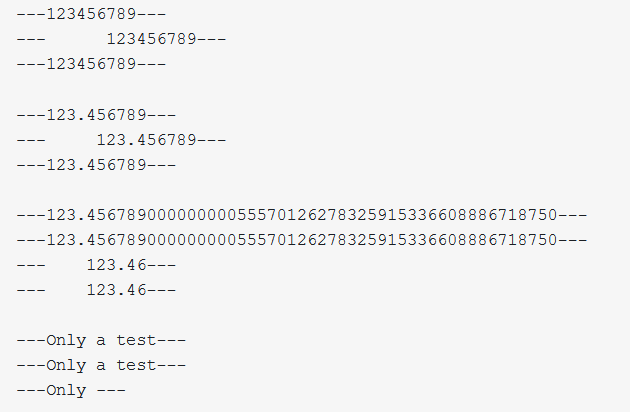
\includegraphics[width=0.4\textwidth]{content/3/chapter5/images/30.png}\\
Applying the width and precision specifiers
\end{center}

\hspace*{\fill} \\ %插入空行
\noindent
\textbf{5.6.1.2.4\hspace{0.2cm} Type}

In general, the compiler deduces the type of the value used. But sometimes, you want to specify the type. These are the most important type specifications:

\begin{itemize}
\item 
Strings: s

\item 
Integers:
\begin{itemize}
\item 
b: binary format

\item 
B: same as b but base Prefix is 0B

\item 
d: decimal format

\item 
o: octal format

\item 
x: hexadecimal format

\item 
X: same as x, but base prefix is 0X
\end{itemize}

\item 
char and wchar\_t:
\begin{itemize}
\item 
b, B, d, o, x, X: such as integers
\end{itemize}

\item 
bool:
\begin{itemize}
\item 
s: true or false

\item 
b, B, d, o, x, X: such as integers
\end{itemize}

\item 
Floating-point:
https://en.cppreference.com/w/cpp/utility/format/formatter
\end{itemize}

When you don’t specify the type, the values are displayed as follows. A string is displayed as a string, an integer in decimal format, a character as a character, and a floating-point value with \href{https://en.cppreference.com/w/cpp/utility/to_chars}{std::to\_chars}.

Thanks to the type specifiers, you can easily display an int in a different number system.

\hspace*{\fill} \\ %插入空行
\noindent
Applying the type specifier
\begin{lstlisting}[style=styleCXX]
// formatType.cpp

#include <fmt/core.h>
#include <iostream>

int main() {

	int num{2020};
	
	std::cout << "default: " << fmt::format("{:}", num) << '\n';
	std::cout << "decimal: " << fmt::format("{:d}", num) << '\n';
	std::cout << "binary: " << fmt::format("{:b}", num) << '\n';
	std::cout << "octal: " << fmt::format("{:o}", num) << '\n';
	std::cout << "hexadecimal: " << fmt::format("{:x}", num) << '\n';

}
\end{lstlisting}

\begin{tcblisting}{commandshell={}}
default:     2020
decimal:     2020
binary:      11111100100
octal:       3744
hexadecimal: 7e4
\end{tcblisting}

\begin{center}
Applying the type specifier
\end{center}

So far, I’ve formatted basics types and strings. Additionally, you can format user-defined types.

\subsubsubsection{5.6.2\hspace{0.2cm} User-Defined Types}

To format a user-defined type, I have to specialize the class \href{https://en.cppreference.com/w/cpp/utility/format/formatter}{std::formatter} for my user-defined type. This means, in particular, I have to implement the member functions parse and format.

\begin{itemize}
\item 
parse:
\begin{itemize}
\item 
Accepts the parse context

\item 
Parses the parse context

\item 
Returns an iterator to the end of the format specification

\item 
Throws a std::format\_error in case of an error
\end{itemize}

\item 
format:
\begin{itemize}
\item 
Gets the value t, which should be formatted, and the format context fc

\item 
Formats t according to the format context

\item 
Writes the output to fc.out()

\item 
Returns an iterator that represents the end of the output
\end{itemize}
\end{itemize}

Let me put the theory into practice and format a std::vector.

\hspace*{\fill} \\ %插入空行
\noindent
\textbf{5.6.2.1\hspace{0.2cm} Formatting a std::vector}

My first specialization of the class std::formatter is as easy as possible. I specify a format specification used for each element of the container.

\hspace*{\fill} \\ %插入空行
\noindent
Applying the format specification to the elements of a std::vector
\begin{lstlisting}[style=styleCXX]
// formatVector.cpp

#include <iostream>
#include <fmt/format.h>
#include <string>
#include <vector>

template <typename T>
struct fmt::formatter<std::vector<T>> {

	std::string formatString;
	
	auto constexpr parse(format_parse_context& ctx) {
		formatString = "{:";
		std::string parseContext(std::begin(ctx), std::end(ctx));
		formatString += parseContext;
		return std::end(ctx) - 1;
	}
	
	template <typename FormatContext>
	auto format(const std::vector<T>& v, FormatContext& ctx) {
		auto out= ctx.out();
		fmt::format_to(out, "[");
		if (v.size() > 0) fmt::format_to(out, formatString, v[0]);
		for (int i= 1; i < v.size(); ++i) fmt::format_to(out, ", " + formatString, v[i]);
		fmt::format_to(out, "]");
		return fmt::format_to(out, "\n" );
	}

};


int main() {

	std::vector<int> myInts{1, 2, 3, 4, 5, 6, 7, 8, 9, 10};
	std::cout << fmt::format("{:}", myInts);
	std::cout << fmt::format("{:+}", myInts);
	std::cout << fmt::format("{:03d}", myInts);
	std::cout << fmt::format("{:b}", myInts);
	
	std::cout << '\n';
	
	std::vector<std::string> myStrings{"Only", "for", "testing", "purpose"};
	std::cout << fmt::format("{:}", myStrings);
	std::cout << fmt::format("{:.3}", myStrings);

}
\end{lstlisting}

The specialization for std::vector (line 8) has the member functions parse (line 13) and format (line 20). parse essentially creates the formatString which is applied to each element of the std::vector (lines 24 and 25). The parse context ctx (line 13) contains the characters between the colon (:) and the closing curly brace (\}). On end, the function returns an iterator to the closing curly brace (\}). The job of the member function format is more interesting. The format context returns the output iterator. Thanks to the output iterator and the function \href{https://en.cppreference.com/w/cpp/utility/format/format_to}{std::format\_to}, the elements of a std::vector are nicely displayed.

The elements of the std::vector (line 35) are formatted in a few ways. Line 36 displays the number, line 37 writes a sign before each number, line 38 aligns them to 3 characters and uses the 0 as a fill character. Line 39 displays them in binary format. The remaining two lines output each string of the std::vector. Finally, line 45 truncates each string to three characters.

\begin{center}
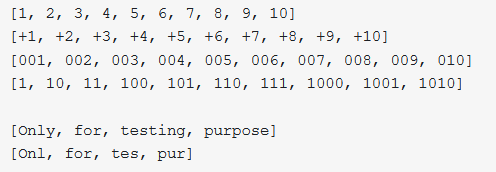
\includegraphics[width=0.4\textwidth]{content/3/chapter5/images/1-8.png}\\
Applying the format specification to the elements of a std::vector
\end{center}

When the std::vector becomes bigger, I want to add a linebreak. For this use case, I extended the syntax of the format specification.

\hspace*{\fill} \\ %插入空行
\noindent
Layouting the elements of a std::vector
\begin{lstlisting}[style=styleCXX]
// formatVectorLinebreak.cpp

#include <algorithm>
#include <iostream>
#include <limits>
#include <numeric>
#include <fmt/format.h>
#include <string>
#include <vector>

template <typename T>
struct fmt::formatter<std::vector<T>> {

	std::string systemFormatString;
	std::string userFormatString;
	int lineBreak{std::numeric_limits<int>::max()};
	
	auto constexpr parse(format_parse_context& ctx) {
		std::string startFormatString = "{:";
		std::string parseContext(std::begin(ctx), std::end(ctx));
		auto posCurly = parseContext.find_last_of("}");
		auto posTab = parseContext.find_last_of("|");
		if (posTab == std::string::npos) {
			systemFormatString = startFormatString + parseContext.substr(0, posCurly + 1);
		}
		else {
			systemFormatString = startFormatString + parseContext.substr(0, posTab) + "}";
			userFormatString = parseContext.substr(posTab + 1, posCurly - posTab - 1);
			lineBreak = std::stoi(userFormatString);
		}
		return std::begin(ctx) + posCurly;
	}

template <typename FormatContext>
auto format(const std::vector<T>& v, FormatContext& ctx) {
	auto out = ctx.out();
	auto vectorSize = v.size();
	if (vectorSize == 0) return fmt::format_to(out, "\n");
	for (int i = 1; i < vectorSize + 1; ++i) {
		fmt::format_to(out, systemFormatString, v[i-1]);
		if ( (i % lineBreak) == 0 ) fmt::format_to(out, "\n");
	}
		return fmt::format_to(out, "\n" );
	}

};

int main() {

	std::vector<int> myInts(100);
	std::iota(myInts.begin(), myInts.end(), 1);
	
	std::cout << fmt::format("{:|20}", myInts);
	std::cout << '\n';
	std::cout << fmt::format("{: |20}", myInts);
	std::cout << '\n';
	std::cout << fmt::format("{:4d|20}", myInts);
	std::cout << '\n';
	std::cout << fmt::format("{:10b|8}", myInts);

}
\end{lstlisting}

Here is how it works. I support an optional | followed by a number to the format specification. The number tells if a line break should be introduced. I search for the optional | symbol and the closing curly brace \}. For robustness reasons, I start in lines 21 and 22 from the end. Thanks to the index of the | symbol and the index of the \}, I can create the strings systemFormatString and useFormatString (lines 24 to 29). The member function format uses the systemFormatString and applies it to each element of the vector. I make a line break when (i \% lineBreak == 0) holds (line 41).

Line 53 displays 20 elements in a row and makes a line break. I can do better. The format specification \{: |20\} (line 55) puts a space before each number. Additionally, line 57 aligns each element to four characters. Finally, the last line displays 8 numbers per line, aligns each element to 8 characters, and displays them: {:10b|8}.

The screenshot shows the readable formated elements of the std::vector.

\begin{center}
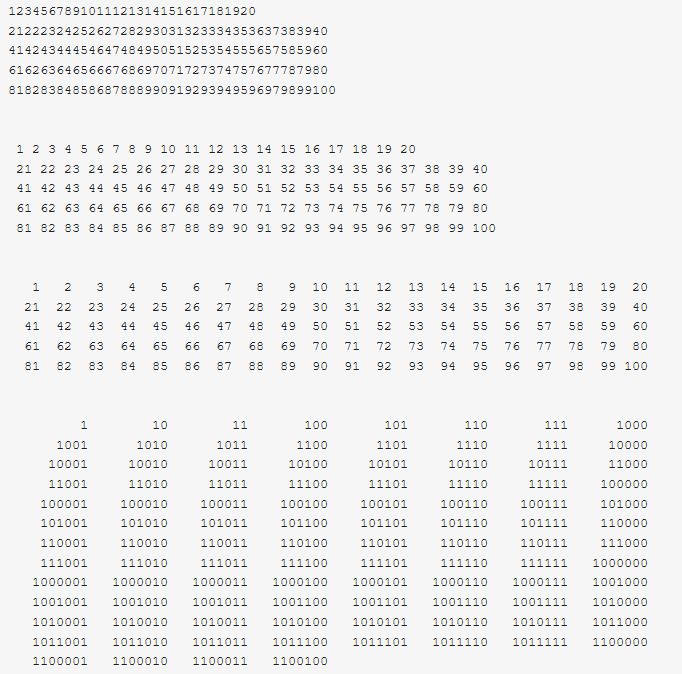
\includegraphics[width=0.4\textwidth]{content/3/chapter5/images/31.png}\\
Applying the format specification and a line break to the elements of a std::vector
\end{center}

\begin{tcolorbox}[breakable,enhanced jigsaw,colback=mygreen!5!white,colframe=mygreen!75!black,title={Distilled Information}]
	
\begin{itemize}
\item 
The formatting library offers a secure and expandable alternative to the printf family and extends the I/O streams.

\item 
The format specification allows you to specify fill letters and text alignment, set the sign, specify the width and the precision of numbers, and specify the data type.

\item 
Thanks to the functions parse and format, the formatting of a user-defined type can be tailored to your needs.
\end{itemize}
	
\end{tcolorbox}

\newpage




